\begin{figure}[ht]
    \centering
        
    \begin{tikzpicture}
\tikzstyle{process}=[draw,rectangle, rounded corners, fill=yellow!20, minimum width=1cm, auto, on grid, minimum height=1cm, align=center]
\tikzstyle{process4}=[draw,font=\small, rectangle, rounded corners,fill=yellow!20, text width=3cm, auto,on grid,align=center]
\tikzstyle{decision}=[draw,font=\small, rectangle, rounded corners,fill=red!20, text width=3cm, auto,on grid,align=center]
\tikzstyle{process2}=[draw,font=\small, rectangle, rounded corners,fill=cyan!20, text width=3cm, auto,on grid,align=center]
\tikzstyle{process3}=[draw, font=\fontsize{5}{4.8}\selectfont,rectangle, rounded corners,fill=gray!20, rotate=-90, auto,on grid,align=center]

\tikzstyle{vecArrow} = [thick, decoration={markings,mark=at position
   1 with {\arrow[semithick]{open triangle 60}}},
   double distance=1.4pt, shorten >= 5.5pt,
   preaction = {decorate},
   postaction = {draw,line width=1.4pt, white,shorten >= 4.5pt}]
\tikzstyle{vecArrow1} = [thick, decoration={markings,mark=at position
   0.9 with {}},
   double distance=1.4pt, shorten >= 5.5pt,
   preaction = {decorate},
   postaction = {draw,line width=1.4pt, white,shorten >= 4.5pt}]
\tikzstyle{innerWhite} = [semithick, white,line width=1.4pt, shorten >= 4.5pt]
\node[inner sep=0pt] (tri) at (3.5,-0.35){{\scalebox{.14}{   
\begin{overpic}[scale=5]{figures/triangulation}
\put(-2,15){$C_L$}
\put(15,12){$X_L$}
\put(0,5){$Y_L$}
\put(92,14){$C_R$}
\put(91,5){$Y_R$}
\put(102,18){$X_R$}
\put(85,27){$f$}
\put(83,33){$c_R$}
\put(17,27){$f$}
\put(12,33){$c_L$}
\put(44,-3){R}
\put(44,13.5){T}
\put(28,9.5){{\fontsize{50}{36}\selectfont Kalman triangulation}}
\put(24,47){$Z_L$}
\put(6,47){$u_L$}
\put(-3,39){$v_L$}
\put(50,59){$P_0$}
\put(63,59){$P_1$}
\put(74,47){$Z_R$}
\put(70,42){$u_R$}
\put(62,33){$v_R$}
\end{overpic}}}};
\node[inner sep=0pt] (1) at (-4,0.5){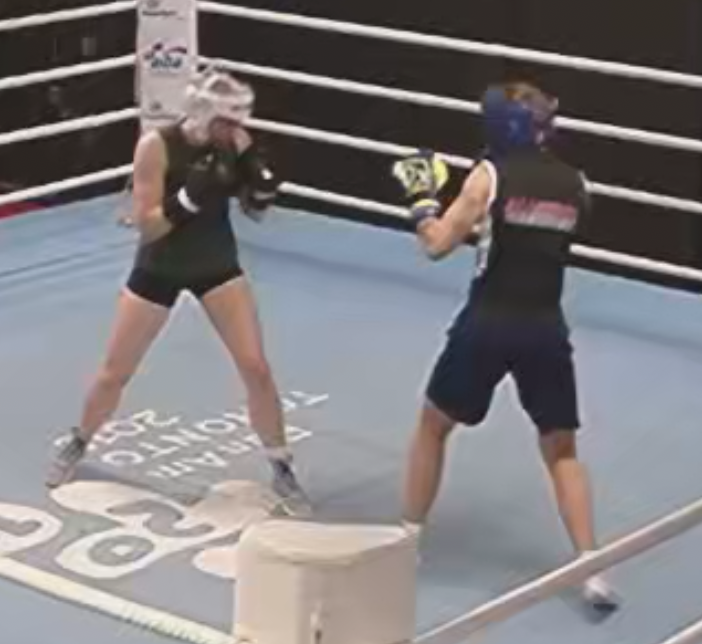
\includegraphics[width=.1\textwidth]{figures/p1.png}};
\node[inner sep=0pt] (2) at (-4,-1.1) {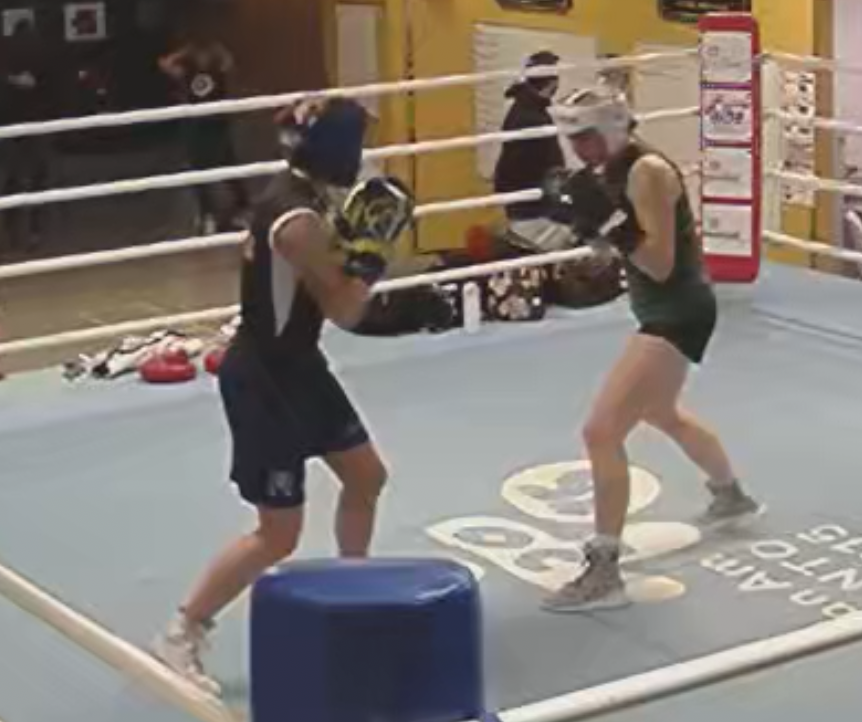
\includegraphics[width=.1\textwidth]{figures/p2.png}};
\node[process] (pose) at (-1,-0.35) {Tracking \\ 2D Pose};
\node[process2] (sort) at (-1,0.75) {\tiny{StrongSort}};
\node[process2] (vitpose) at (-1,-1.5) {\tiny{ViTPose}};
\draw[vecArrow] (vitpose) to (pose);
\draw[vecArrow] (sort) to (pose);
\draw[vecArrow] (-3.25,-0.35) tonode[anchor=south] {\scriptsize{calibrated}} (pose);
\node[process3] (epipolar) at (0.4,-0.35){epipolar constraints};
\draw[vecArrow] (pose) to  (epipolar);
\draw[vecArrow] (epipolar) to  (tri);
\node[process] (kinematics) at (8,-0.35) {Kinematics\\Optimization};
\node[process2] (prior) at (8,0.75) {\tiny{CMU GMM Prior}};
\node[process2] (loss) at (8,-1.5) {\tiny{$L_{2D}+L_{3D}+L_{\beta}$}};
\draw[vecArrow] (loss) to (kinematics);
\draw[vecArrow] (prior) to (kinematics);
\draw[vecArrow] (tri) to (kinematics);

\node[inner sep=0pt] (smpl2) at (11,-0.35) {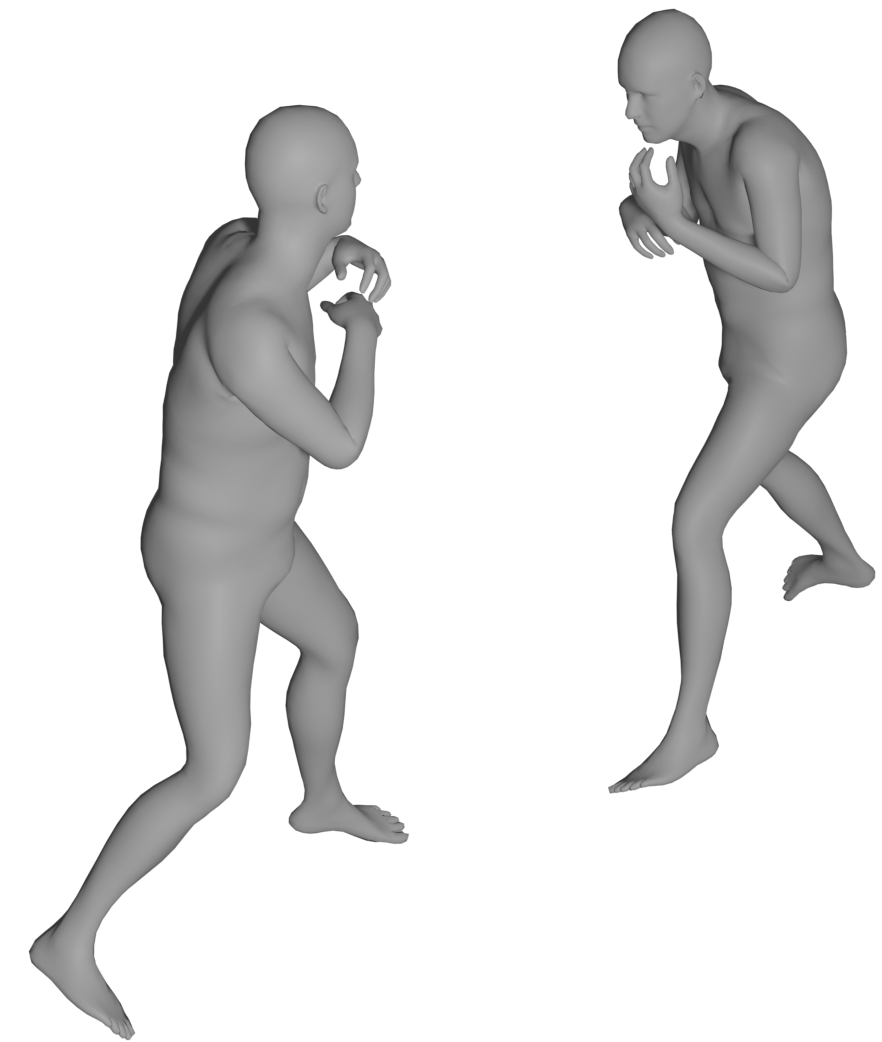
\includegraphics[width=.1\textwidth]{figures/smpl2.png}};
\draw[vecArrow] (kinematics) to (smpl2);
\node[inner sep=0pt] (smpl) at (-4,-3){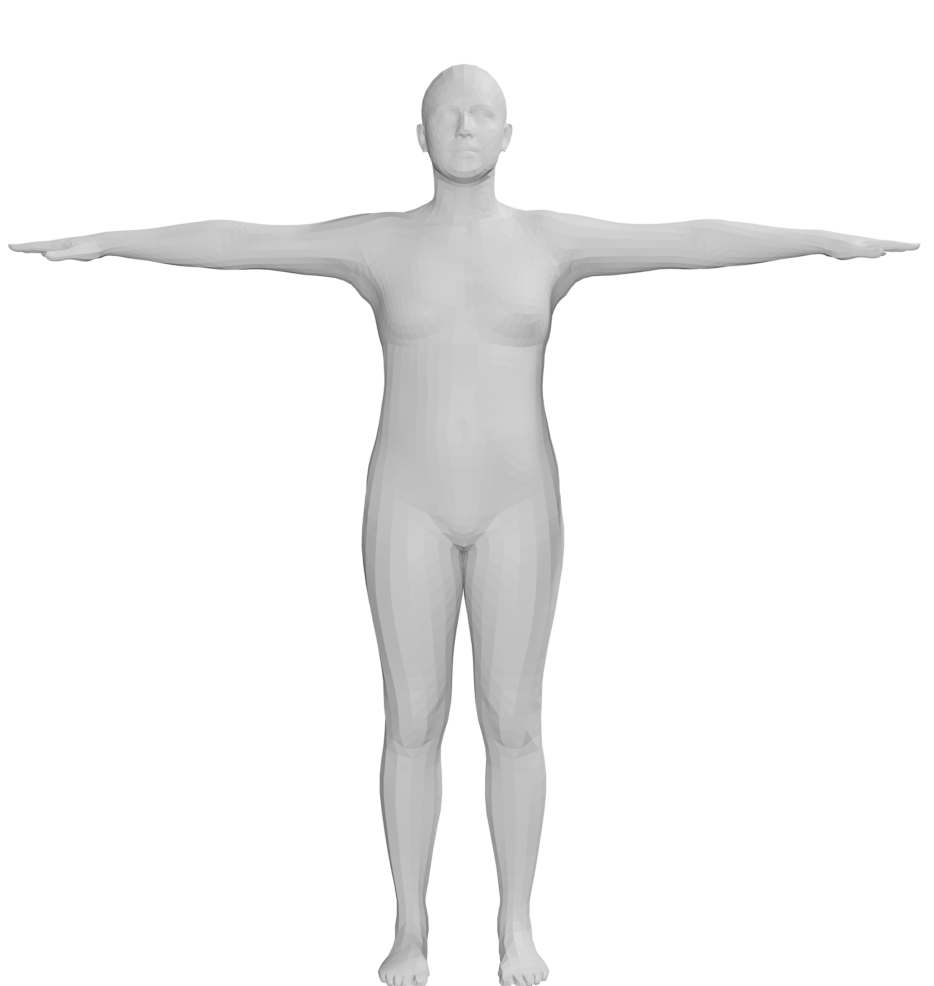
\includegraphics[width=.1\textwidth]{figures/smpl.png}};
\node[decision] (retarget) at (-1.2,-3) {\scriptsize{$\beta$\_Humanoid Generator }};
\draw[vecArrow] (smpl) to (retarget);

\node[inner sep=0pt] (humanoid) at (1.5,-3){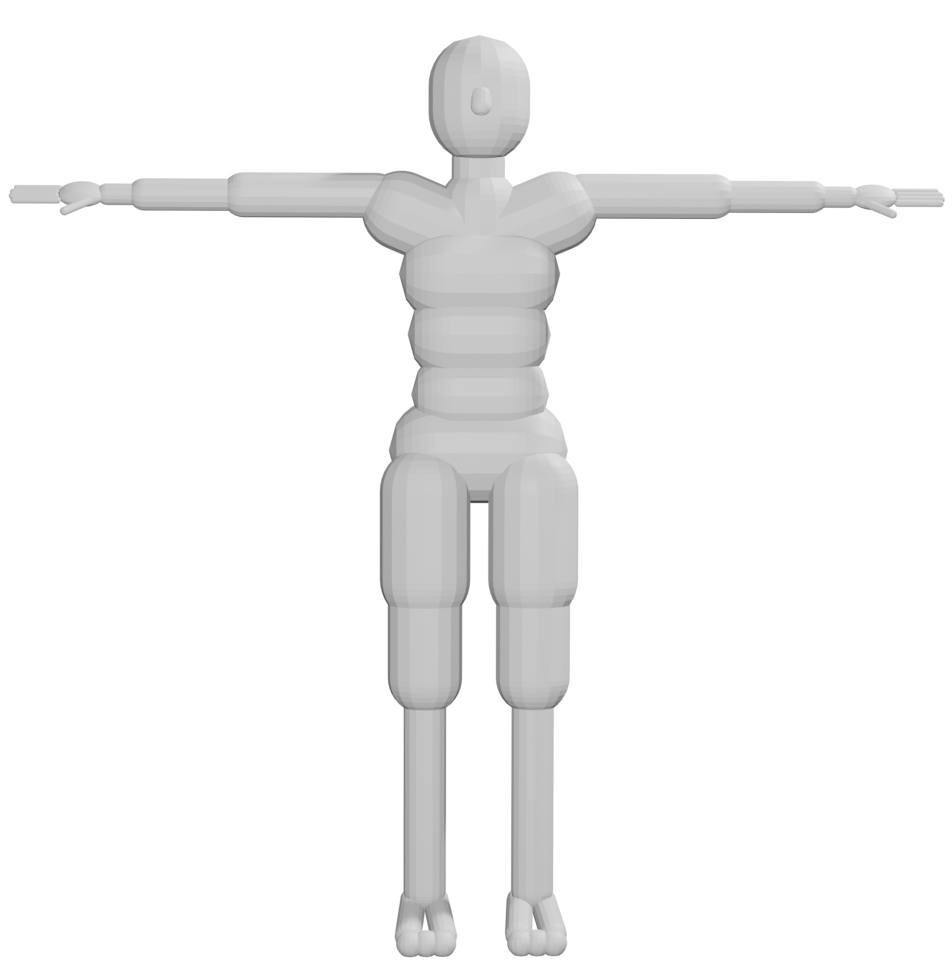
\includegraphics[width=.1\textwidth]{figures/humanoid.png}};
\draw[vecArrow] (retarget) to (humanoid);
\node[inner sep=0,minimum size=0] (k) at (4.4, -2) {};
\node[process2] (lqr) at (4.4,-3) {LQR Single-Person Optimization};
\draw[vecArrow] (humanoid) to (lqr);
\draw[vecArrow1] (smpl2) |- (4.155,-2);
\draw[vecArrow] (4.4, -1.975) tonode[anchor=west] {\tiny{$qpos$,$qvel$,$mpos$}} (lqr);
\node[inner sep=0,minimum size=0] (k1) at (-1.2, -2.15) {};
\draw[vecArrow1] (4.4, -2.15) to (-1.445, -2.15);
\draw[vecArrow] (-1.2, -2.125) tonode[anchor=west] {\scriptsize{$\beta$}} (retarget);
\draw[innerWhite] (smpl2) |- (4.22,-2);
\draw[innerWhite] (k) -- (lqr);
\draw[innerWhite] (4.4, -2.15) -- (-1.38, -2.15);
\node[process4] (lqr2) at (8,-3) {Direct Multi-person Optimization};
\draw[vecArrow] (lqr) to (lqr2);
\node[inner sep=0pt] (final) at (11,-3){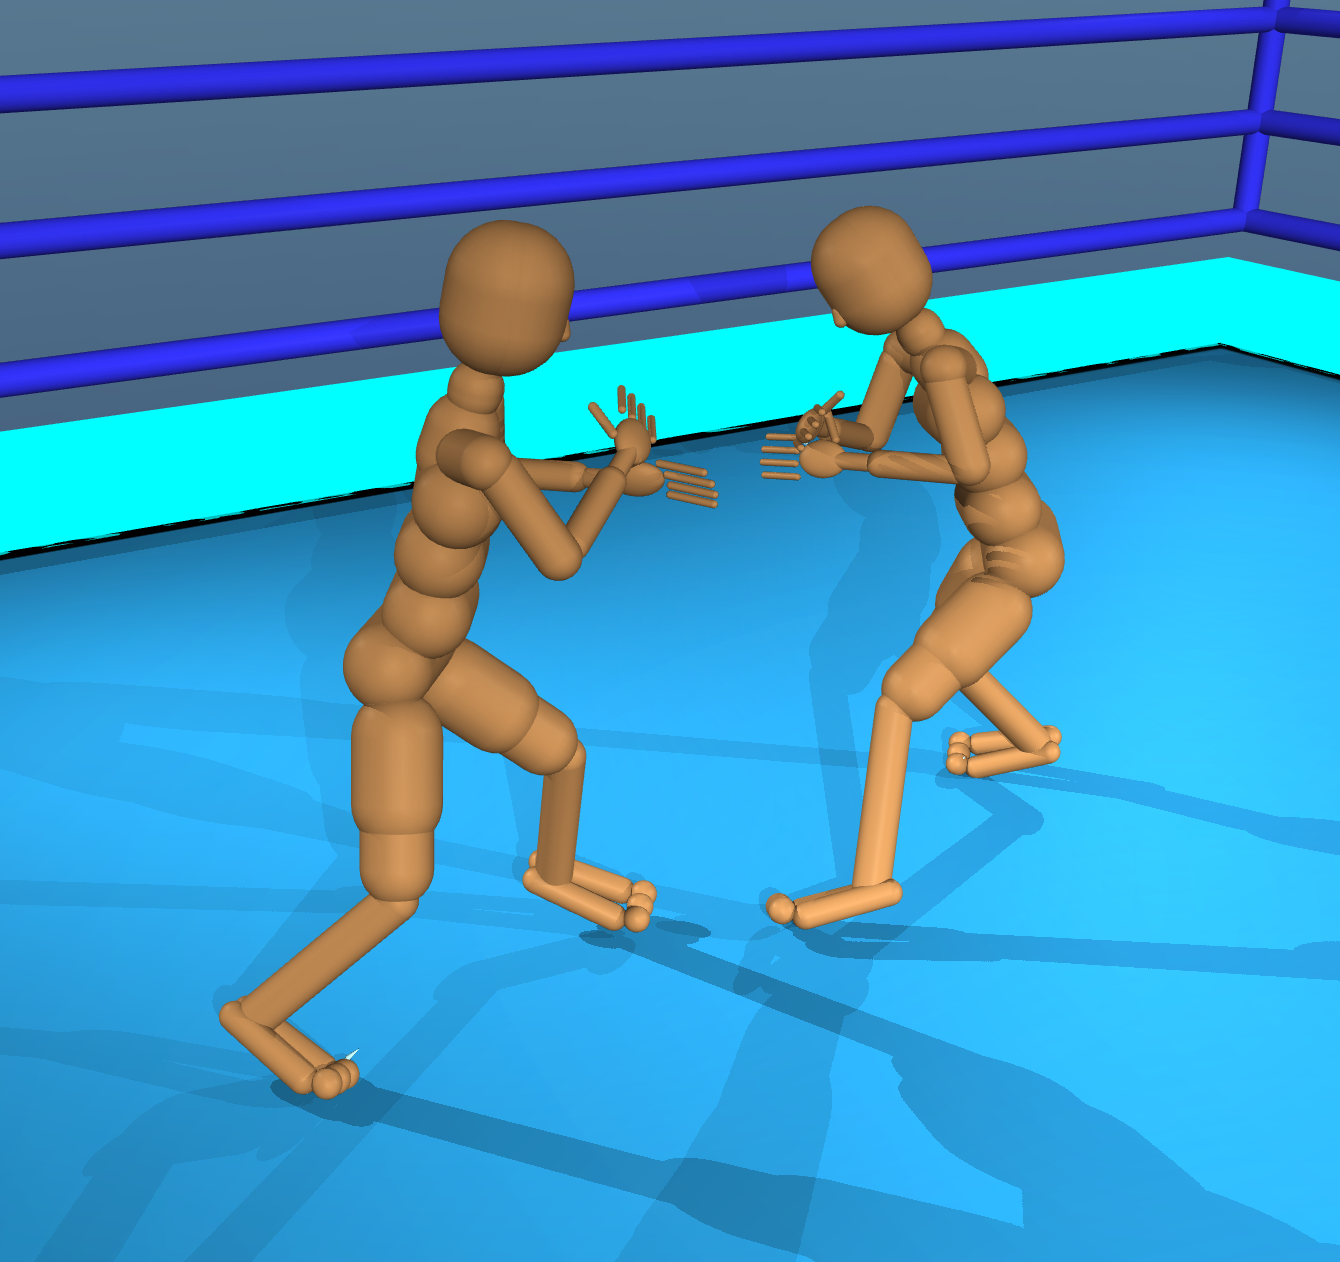
\includegraphics[width=.125\textwidth]{figures/final.png}};
\draw[vecArrow] (lqr2) to (final);

\end{tikzpicture}
\caption{\textbf{Pipeline structure.} The pipeline start with a tracking method for producing the bounding boxes and robust tracking IDs for all individuals in the scene which will be used for creating 2D poses using ViTPose\cite{xu2022vitpose}. The 2D poses of the target serve as input for the Kalman weighted triangulator, which filters the noisy keypoints by its prediction . Next Kinematics optimization incorporates the 2D, 3D key-points and prior information to create the SMPL parameters. In each iteration, 3D joints are optimized by 2D reprojection error, considering the 2D confidences. The Kinematics optimization output will be used for automatic $\beta$ humanoid generation and Dynamics optimization of the pose. The 3D joint positions of the humanoid are used as a reference pose for a model predictive controller, utilizing the LQR optimizer \cite{howell2022} to correct the artifacts in the motion. At the end we use direct multi-person optimization to correct the intra person artifacts} 
\label{fig:3d}
\end{figure}
